\section{Implementazione}\label{sec:implementazione}

\subsection{Modellazione circuito}
Come accennato nella Sez. \ref{sec:background}, la rappresentazione 
delle immagini viene implementata attraverso la tecnica QPIE. 
Per farlo, si utilizza una matrice associata all'immagine di partenza
i cui elementi corrispondono ai valori d'intensità dei pixel.
Su questa matrice viene effettuato un processo di normalizzazione.
Il risultato è un vettore di stato, composto da ampiezze di
probabilità relative allo stato quantistico del sistema. In Fig.~\ref{fig:16x16intensity_img} è mostrata un'immagine di 
dimensione $16 \times 16$ dopo la normalizzazione. Ogni pixel 
con valore ``alto'' rappresenta un risultato della misurazione 
che può essere generata dal circuito con ampiezza di probabilità $0.14$.

Dato un vettore di stato composto da $2^n$ elementi, 
il passo successivo consiste nella creazione di un circuito a $n+1$ qubit, 
compreso quello ausiliario o \textit{ancilla qubit}.
La costruzione avviene tramite applicazione di procedure Qiskit \textit{built-in} 
all'oggetto che rappresenta il circuito.
Nel Cod. \ref{cod:circuit} vengono mostrate le operazioni svolte durante
questa fase, oltre all'applicazione dei gate Hadamard e della matrice 
di shift $D_{2^{n+1}}$.

\begin{figure}
    \centering
    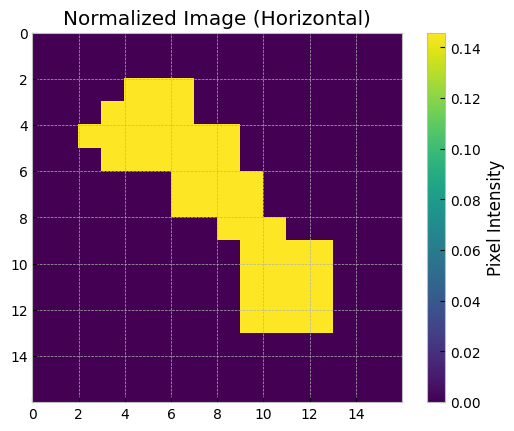
\includegraphics[width=0.4\textwidth]{16x16.png}
    \caption{Immagine normalizzata (ampiezze di probabilità).}
    \label{fig:16x16intensity_img}
\end{figure}

\begin{lstlisting}[language=Python, 
    caption={Creazione dei circuiti per lo scan orizzontale e verticale.}, label=cod:circuit]
# Convert the raw pixel values to probability amplitudes
def amplitude_encode(img_data):
    
    # Calculate the RMS value
    rms = np.sqrt(np.sum(np.sum(img_data**2, axis=1)))
    
    # Create normalized image
    image_norm = []
    for arr in img_data:
        for ele in arr:
            image_norm.append(ele / rms)
        
    # Return the normalized image as a numpy array
    return np.array(image_norm)
# Initialize some global variable for number of qubits
data_qb = math.floor(math.log2(height * width))
anc_qb = 1
total_qb = data_qb + anc_qb

# Initialize the amplitude permutation unitary
D2n_1 = np.roll(np.identity(2**total_qb), 1, axis=1)

# Create the circuit for horizontal scan
qc_h = QuantumCircuit(total_qb)
qc_h.initialize(image_norm_h, range(1, total_qb))
qc_h.h(0)
qc_h.unitary(D2n_1, range(total_qb))
qc_h.h(0)
display(qc_h.draw('mpl', fold=-1))

# Create the circuit for vertical scan
qc_v = QuantumCircuit(total_qb)
qc_v.initialize(image_norm_v, range(1, total_qb))
qc_v.h(0)
qc_v.unitary(D2n_1, range(total_qb))
qc_v.h(0)
display(qc_v.draw('mpl', fold=-1))

# Combine both circuits into a single list
circ_list = [qc_h, qc_v]
\end{lstlisting} 

\begin{figure}[ht]
    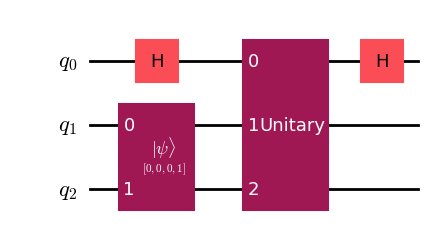
\includegraphics[width=0.4\textwidth]{circuit.png}
    \caption{Circuito per scan orizzontale su immagine $2 \times 2$.}
    \label{fig:circuit}
\end{figure}

Il circuito ottenuto per un'immagine $2 \times 2$ è mostrato in Fig.~\ref{fig:circuit}.
Come si può notare, l'operazione relativa alla matrice di shift (chiamata anche
\emph{decrement gate}) è 
rappresentata come una black-box di cui non si conoscono i dettagli.
È possibile, tuttavia, utilizzare una rappresentazione più a basso livello 
composta solo da porte logiche $H$, $X$, $CX$ e $CCX$ (Toffoli gate).
Questa casistica è presentata solo per immagini di piccole dimensioni, per limitare il 
rumore presente durante l'esecuzione. La parte di circuito a sinistra della barriera
corrisponde alla preparazione dello stato $\ket{\psi}$: in questo caso, si tratta 
di impostare a 1 il valore del qubit $q_1$.

\begin{figure}[ht]
    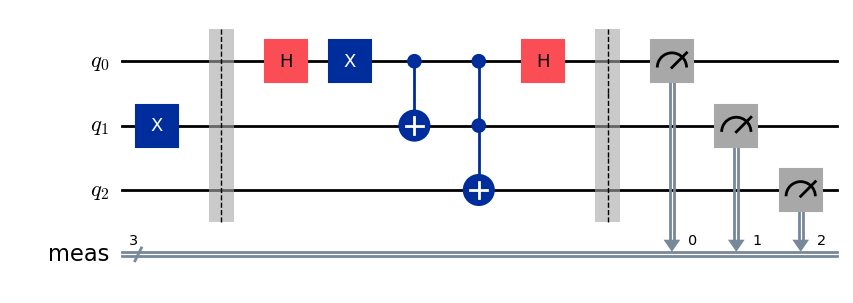
\includegraphics[width=0.4\textwidth]{low-level.png}
    \caption{Versione del circuito a basso livello.}
		\label{fig:circuito-2x2}
\end{figure}

\subsection{Simulazioni ideali}
Le misurazioni vengono svolte inizialmente tramite simulazione, utilizzando 
il framework \texttt{statevector\_simulator}. In questo meccanismo si lavora su 
una simulazione di un circuito quantistico ideale, ovvero senza effetti collaterali come
fluttuazioni termiche, imperfezioni delle porte quantistiche, interazione con l'ambiente 
o altre tipologie di \textit{rumore}.
In un'esecuzione realistica, tuttavia, occorre tenere in considerazione
tali problematiche che, molto spesso, complicano pesantemente
il circuito e richiedono tecniche non banali di \textit{mitigazione dell'errore}.

\subsection{Gestione degli errori}
Si possono eseguire delle misurazioni significative utilizzando modelli 
di rumore forniti dalla classe \texttt{NoiseModel} di Qiskit. 
Per farlo, ci si connette ad uno dei backend disponibili, per esempio 
\texttt{ibm\_kyiv} in questo caso. Da questo backend si estrapolano le 
informazioni necessarie all'esecuzione, ovvero:
\begin{itemize}
	\item \emph{noise model}: rappresenta il modello di rumore considerato;
		\item \emph{basis gates:} rappresentano le porte disponibili sull'hardware;
		\item \emph{coupling map:} rappresenta la disposizione fisica dei qubit sull'hardware.
\end{itemize}
Dopo aver definito queste proprietà, si prosegue con le misurazioni 
ripetute del circuito. Nel Cod. \ref{cod:noise} sono mostrati 
i comandi per estrarre le informazioni necessarie e per eseguire 
in maniera iterativa le misurazioni del circuito, salvando i risultati 
come statistiche da elaborare in una fase successiva.

\begin{lstlisting}[language=Python, 
caption={Estrapolazione del modello di rumore dal backend \texttt{ibm\_kyiv}.}, label=cod:noise]
service = QiskitRuntimeService(channel="ibm_quantum", token="<token>")
backend = service.backend("ibm_kyiv")
noise_model = NoiseModel.from_backend(backend)
coupling_map = backend.configuration().coupling_map
basis_gates = noise_model.basis_gates
# Unione dei circuiti in una lista unica
circ_list = [qc_h, qc_v]
# Array per memorizzare i risultati intermedi
results_list = []

# Iterazione per variare il numero di shots
for exponent in range(8, 20, 2):
    shots = 2 ** exponent
    print(f"Running simulation with {shots} shots...")
    
    # Simulazione
    result = backend.run(circ_list, shots=shots).result()
    
    # Estrazione conteggi
    counts_h = result.get_counts(qc_h)
    counts_v = result.get_counts(qc_v)
    
    # Salvataggio risultati 
    results_list.append({
        'shots': shots,
        'counts_h': counts_h,
        'counts_v': counts_v
    })
\end{lstlisting}

%% spostare nei risultati
% \begin{figure}
%     \centering
%     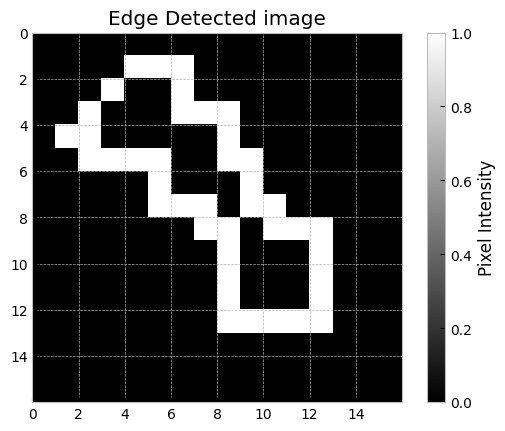
\includegraphics[width=0.4\textwidth]{ideal.png}
%     \caption{Edge detection tramite simulazione}
%     \label{fig:ideal}
% \end{figure}
